\chapter{Общая модель стандартного генетического алгоритма}\label{StandardGA:section_commonmodel}

Генетический алгоритм можно представить как некий стохастический оператор, который на выходе выдает \textbf{субоптимальное} решение $ \bar{x}_{submax} $ и значение функционала от этого решения $ f\left( \bar{x}_{submax}\right)  $. То есть мы можем записать, что

\begin{equation}
\label{StandardGA:eq:commommodelGA}
\left( \begin{array}{c} \bar{x}_{submax} \\ f\left( \bar{x}_{submax}\right)\end{array}\right)=GeneticAlgorithm\left( \begin{array}{c} X \\ f\left( \bar{x}\right) \\ g_i\left( \bar{x}\right) \\ h_j\left( \bar{x}\right) \\ Parameters \end{array}\right),
\end{equation}

где $i=\overline{1,m_1}, j=\overline{1,m_2}$,

$GeneticAlgorithm$ --- непосредственно сам генетический алгоритм как оператор,

$Parameters$ --- параметры генетического алгоритма, которые определяет пользователь (будут рассмотрены ниже).

В виде схемы это можно представить так:

\begin{figure} [h] 
  \center
  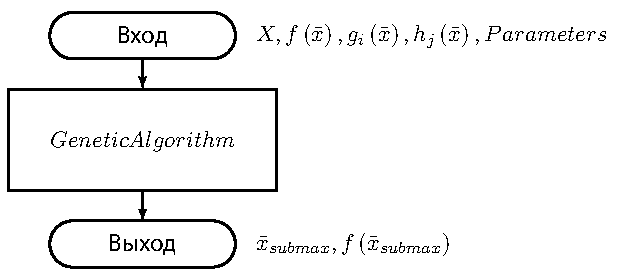
\includegraphics [scale=1] {GABlack}
  \caption{Модель черного ящика генетического алгоритма} 
  \label{StandardGA:img:GABlack}  
\end{figure}

Как было отмечено выше, стандартный генетический алгоритм (сГА) решает задачу оптимизации, как на бинарных строках, так и на вещественных. Поэтому стандартный генетический алгоритм включает в себя два алгоритма:

\begin{itemize}
\item стандартный генетический алгоритм на бинарных строках ($ BinaryGeneticAlgorithm $);
\item стандартный генетический алгоритм на вещественных строках.
\end{itemize}

При этом сГА на вещественных строках включает в себя сГА на бинарных строках, а также блок преобразования задачи вещественной оптимизации к задаче бинарной оптимизации и блок преобразования полученного бинарного решения к вещественному.

По этой причине вектор параметров сГА состоит из двух частей:

\begin{equation}
\label{StandardGA:eq:ParametersGA}
Parameters=\left( \begin{array}{c} ParametersOfBinaryGA \\ ParametersOfConvertingIntoBinaryGA\end{array}\right).
\end{equation}

Здесь $ ParametersOfBinaryGA $ --- параметры стандартного генетического алгоритма на бинарных строках, а $ ParametersOfConvertingIntoBinaryGA $ --- параметры преобразования задачи оптимизации на вещественных векторах к задаче оптимизации на бинарных векторах. В случае если в конкретном случае решается задача бинарной оптимизации, то блок параметров $ ParametersOfConvertingIntoBinaryGA $ можно опустить.

Построим общую схему сГА, учитывая вышесказанное (рис. \ref{StandardGA:img:GACommonSheme}).

\begin{figure} [h] 
  \center
  \includegraphics [scale=0.7] {GACommonSheme}
  \caption{Общая модель стандартного генетического алгоритма} 
  \label{StandardGA:img:GACommonSheme}  
\end{figure}

Распишем ее в виде алгоритма $ GeneticAlgorithm $:

\begin{algorithm}
\caption{Алгоритм $ GeneticAlgorithm $ (Часть 1)}\label{StandardGA:alg:GeneticAlgorithm}
\begin{algorithmic}

\State \textbf{Начало алгоритма}
\If{$ X $ представляет собой множество вещественных векторов}
\BeginBlock \parbox[t]{\dimexpr\linewidth-\algorithmicindent-\algorithmicindent-\algorithmicindent-\algorithmicindent-\algorithmicindent-\algorithmicindent}{\textbf{\textit{Преобразование задачи вещественной оптимизации в задачу бинарной оптимизации:}}\strut}
\State Выполнить:\begin{flalign*}
&\left( \begin{array}{c} X_{B} \\ f_B\left( \bar{x}_{B}\right)  \\ {g_i}_B\left( \bar{x}_B\right) \\ {h_j}_B\left( \bar{x}_B\right) \\ ParametersOfBinaryGA\end{array}\right)=\\
&=ConvertingIntoBinaryGA\left( \begin{array}{c} X \\ f\left( \bar{x}\right) \\ g_i\left( \bar{x}\right) \\ h_j\left( \bar{x}\right) \\ ParametersOfBinaryGA \\ ParametersOfConvertingIntoBinaryGA \end{array}\right);
\end{flalign*}
\EndBlock
\EndIf
\BeginBlock \parbox[t]{\dimexpr\linewidth-\algorithmicindent-\algorithmicindent-\algorithmicindent-\algorithmicindent-\algorithmicindent}{\textbf{\textit{Выполнение стандартного генетического алгоритма на бинарных строках:}}\strut}
\State \parbox[t]{\dimexpr\linewidth-\algorithmicindent}{Если решается задача бинарной оптимизации, то подается вектор входных параметров самого алгоритма $ GeneticAlgorithm $ (без $ ParametersOfConvertingIntoBinaryGA $, если он присутствует), иначе подается преобразованный вектор, полученный на предыдущем шаге:\strut}
\State $ A=\left\lbrace \begin{array}{l}
\left( \begin{array}{c} X \\ f\left( \bar{x}\right)  \\ {g_i}_B\left( \bar{x}\right) \\ {h_j}\left( \bar{x}\right) \\ ParametersOfBinaryGA\end{array}\right), \mbox{ где } X \mbox{ --- множество бинарных векторов};\\ 
\left( \begin{array}{c} X_{B} \\ f_B\left( \bar{x}_{B}\right)  \\ {g_i}_B\left( \bar{x}_B\right) \\ {h_j}_B\left( \bar{x}_B\right) \\ ParametersOfBinaryGA\end{array}\right), \mbox{ где } X  \mbox{ --- множество вещественных векторов.}
\end{array}\right. $

\State  $ \left( \begin{array}{c} \bar{x}{{}_{submax}}_B \\ {f\left( \bar{x}_{submax}\right)}_B \end{array}\right)=BinaryGeneticAlgorithm \left(  A \right)  $;
\EndBlock

\BeginBlock \textbf{\textit{Тип задачи:}}
\State Используем информацию, полученную на этапе «Анализ типа задачи»;
\If{$ X $ представляет собой множество вещественных векторов}
\State \Return ${\left( \bar{x}_{submax}; f\left( \bar{x}_{submax}\right) \right)}^\mathrm{T} $;
\EndIf
\EndBlock


\State \textit{Продолжение ниже}
  \algstore{bkbreak}
  
\end{algorithmic}
\end{algorithm}

\begin{algorithm}
\caption{Алгоритм $ GeneticAlgorithm $ (Часть 2)}
\begin{algorithmic}
\algrestore{bkbreak}
\State \textit{Начало выше}

\BeginBlock \textbf{\textit{Преобразование бинарного решения в вещественное:}}
\State $ \left( \begin{array}{c} \bar{x}_{submax} \\ f\left( \bar{x}_{submax}\right)\end{array}\right)=BinaryToReal \left( \begin{array}{c} \bar{x}{{}_{submax}}_B \\ {f\left( \bar{x}_{submax}\right)}_B \\ ParametersOfConvertingIntoBinaryGA \end{array}\right)  $;
\State \Return ${\left( \bar{x}_{submax}; f\left( \bar{x}_{submax}\right) \right)}^\mathrm{T} $;
\EndBlock


\State \textbf{Конец алгоритма}
\end{algorithmic}
\end{algorithm}

Операторы $ ConvertingIntoBinaryGA $ и $ BinaryToReal $ рассматриваются в главе \ref{StandardGA:section_realga}. До него рассматривается только стандартный генетический алгоритм на бинарных строках.

\textbf{Замечание.} Существует вещественный генетический алгоритм, который работает непосредственно с вещественными строками без приведения к задаче бинарной оптимизации. В данном Стандарте он не рассматривается.


\clearpage